\section{Versuchsaufbau/-durchführung}
Zur experimentellen Überprüfung der Bragg-Bedingung sowie der quantitativen Untersuchung der Spektren wird der Aufbau nach Abbildung
\ref{fig: aufbau} verwendet. Die Apparatur besteht prinzipiell aus einer Kupferröntgenröhre, einem schwenkbaren Kristall und einem
Geiger-Müller-Zählrohr. Die zeitliche Justage der Drehwinkel, sowei die Datenaufnahme erfolgt mit einer
Messsoftware. Der Aufbau ermöglicht somit eine Untersuchung der Intensität in Abhängigkeit von der Energie
der Röntgenstrahlung.
\begin{figure}
  \centering
  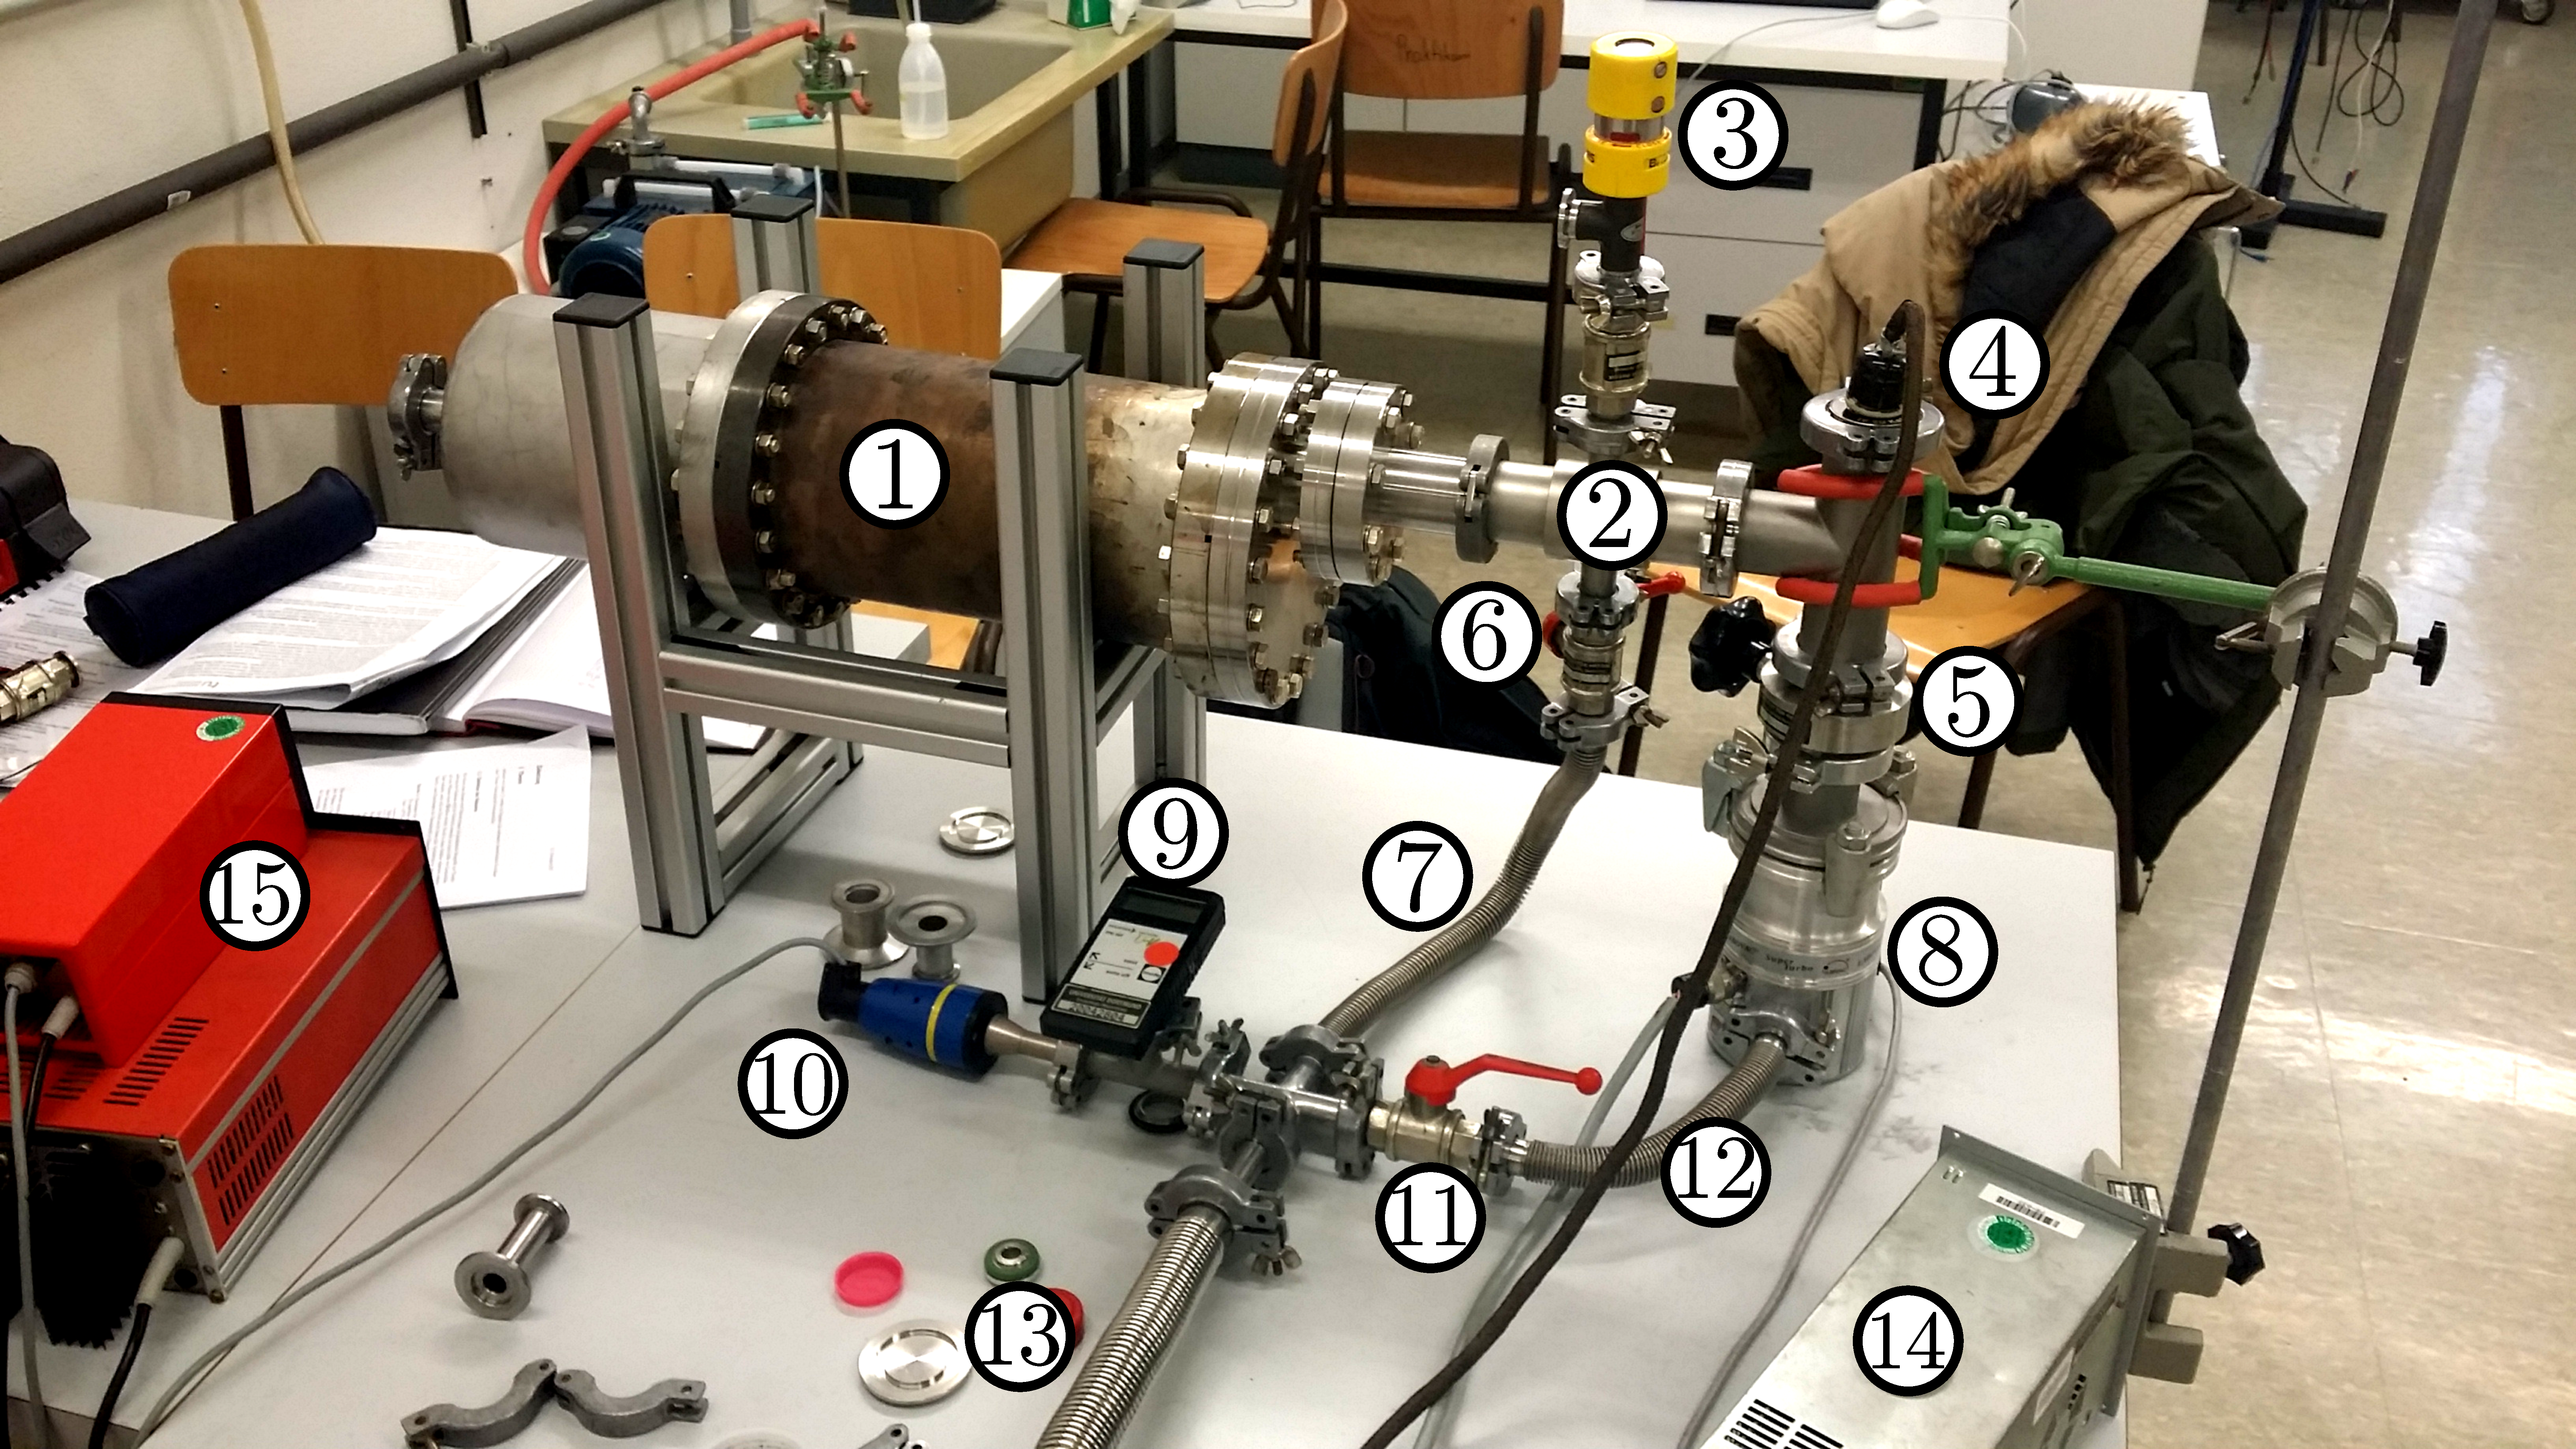
\includegraphics[width = 0.8\textwidth]{pics/aufbau.png}
  \caption{Darstellung der verwendeten Messaparatur zur Untersuchung von Röntgenemission und -absorption \cite{}.}
  \label{fig: aufbau}
\end{figure}
\subsection{Überprüfung der Braggsoftware}

\subsection{Emissionspektrum}

\subsection{Absorptionsspektrum}
